\documentclass{article}

% if you need to pass options to natbib, use, e.g.:
%     \PassOptionsToPackage{numbers, compress}{natbib}
% before loading neurips_2018

% ready for submission
% \usepackage{neurips_2018}

% to compile a preprint version, e.g., for submission to arXiv, add add the
% [preprint] option:
%     \usepackage[preprint]{neurips_2018}

% to compile a camera-ready version, add the [final] option, e.g.:
     \usepackage[final]{neurips_2018}

% to avoid loading the natbib package, add option nonatbib:
%     \usepackage[nonatbib]{neurips_2018}

\usepackage[utf8]{inputenc} % allow utf-8 input
\usepackage[T1]{fontenc}    % use 8-bit T1 fonts
\usepackage{hyperref}       % hyperlinks
\usepackage{url}            % simple URL typesetting
\usepackage{booktabs}       % professional-quality tables
\usepackage{amsfonts}       % blackboard math symbols
\usepackage{nicefrac}       % compact symbols for 1/2, etc.
\usepackage{graphicx}
\usepackage{microtype}      % microtypography
\usepackage{amsmath}
\usepackage{algorithm}
\usepackage{algpseudocode}


\title{CSCI-635 Final Project\\Playing Atari with Deep Reinforcement Learning\\(DeepMind, 2013)}

% The \author macro works with any number of authors. There are two commands
% used to separate the names and addresses of multiple authors: \And and \AND.
%
% Using \And between authors leaves it to LaTeX to determine where to break the
% lines. Using \AND forces a line break at that point. So, if LaTeX puts 3 of 4
% authors names on the first line, and the last on the second line, try using
% \AND instead of \And before the third author name.

\author{%
  Benjamin Piro \\
  % \thanks{Use footnote for providing further information
  %   about author (webpage, alternative address)---\emph{not} for acknowledging
  %   funding agencies.} \\
  CS BS/MS Student\\
  Rochester Institute of Technology\\
  Rochester, NY 14623 \\
  \texttt{brp8396@rit.edu} \\
  % examples of more authors
   \And
   Brandon Kirincich \\
   CS BS/MS Student \\
  Rochester Institute of Technology\\
  Rochester, NY 14623 \\
   \texttt{bjk3435@rit.edu} \\
   \And
   Hanna Koh \\
   CS BS/MS Student \\
  Rochester Institute of Technology\\
  Rochester, NY 14623 \\
   \texttt{hjk5643@rit.edu} \\
  % \AND
  % Coauthor \\
  % Affiliation \\
  % Address \\
  % \texttt{email} \\
  % \And
  % Coauthor \\
  % Affiliation \\
  % Address \\
  % \texttt{email} \\
  % \And
  % Coauthor \\
  % Affiliation \\
  % Address \\
  % \texttt{email} \\
}

\begin{document}
% \nipsfinalcopy is no longer used

\maketitle
\begin{abstract}
  \vspace{-3cm}We give an in-depth introduction to the fundamentals of value-based reinforcement learning in order to understand the developments and contributions of a seminal Deep Reinforcement Learning paper. The paper in question, titled "Playing Atari with Deep Reinforcement Learning" published by DeepMind Technologies in 2013 \cite{dqn}, introduces the first state-of-the-art deep reinforcement learning algorithm, \textit{Deep Q-Networks} (DQN), which was capable of achieving human-level performance on multiple Atari 2600 games without pre-processing states through manual feature-extraction. Since its inception, DQN has caused a resurgence of deep reinforcement learning research, leading to various modern state-of-the-art algorithms such as DreamerV3, Soft Actor-Critic (SAC), Twin-Delayed Deep Deterministic Policy Gradients (TD3), Trust-Region Policy Optimization (TRPO), and Proximal Policy Optimization (PPO) \cite{SpinningUp2018}.
\end{abstract}

\pagebreak
\tableofcontents



\pagebreak
\section{Introduction}

Machine learning has traditionally focused on two paradigms: \textbf{supervised learning}, where models learn from labeled examples, and \textbf{unsupervised learning}, which learns underlying patterns or structures within data without explicit labels. While these approaches are powerful, they often require large, human-constructed datasets which do not inherently address time-dependent control tasks.

\textbf{Reinforcement Learning (RL)} takes a different approach. Instead of passively learning from fixed data, RL involves a learner (called an \textbf{agent}) actively interacting with its environment to achieve a goal. The agent learns through \textbf{trial and error}---inspired by human learning, in which successful actions are reinforced and suboptimal ones are penalized. This ability to learn from sequential feedback makes RL particularly suited to optimal control or path learning problems, where a focus is put on making decisions over time which maximize a long-term reward \cite{Sutton1998}.

In 2013, DeepMind introduced a ground-breaking paper that demonstrated the potential of combining the representational power of \textbf{deep neural networks} with the trial-and-error approach of reinforcement learning. This work introduced the \textbf{Deep Q-Networks (DQN)} algorithm, which enabled an agent to achieve human-level performance on a diverse set of Atari 2600 games \cite{dqn}.

Understanding the significance of this paper requires some foundational knowledge of reinforcement learning. At its core, the DQN algorithm solved key challenges in reinforcement learning by leveraging neural networks as function approximators, allowing the agent to generalize unseen experiences (or 1-step transitions) in a \textbf{Markov Decision Process (MDP)}. This innovation was pivotal in bridging the gap between traditional reinforcement learning methods, such as \textbf{Q-Learning}, which struggled with scalability, and modern machine learning techniques capable of handling high-dimensional data and complex tasks.

In this paper, we start off by introducing the fundamentals of reinforcement learning to provide the necessary context for understanding DeepMind's contributions. We then explore the DQN algorithm and discuss how it represents a significant advancement in reinforcement learning by demonstrating the potential of deep neural networks to approximate action-value functions and the use of an experience replay buffer to enhance data efficiency. These innovations enable agents to effectively learn and perform well in complex, simulated environments.

\section{Background Information}

This section provides an in-depth introduction to the fundamentals of reinforcement learning. Shown later, the Deep Q-Networks (DQN) algorithm and content of the DeepMind paper require only a general understanding of value-based reinforcement learning methods which use deterministic action policies. Therefore this section will not cover policy-gradient methods, stochastic action policies, or model-based methods in depth, as their respective explanations ultimately deviate from the educational goals of this paper. \cite{MutualInformationRLByTheBook}.

\begin{figure}[H]
    \centering
    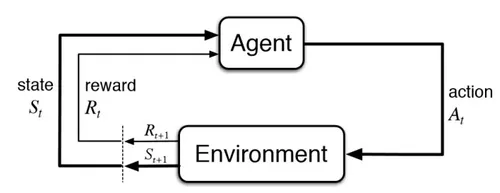
\includegraphics[width=0.75\linewidth]{image.png}
    \caption{Reinforcement Learning Markov Decision Process}
    \label{fig:rlloop}
\end{figure}

\subsection{Introducing Reinforcement Learning}

We start off by defining the key components which make up the problem statement of reinforcement learning (Figure \ref{fig:rlloop}). The \textbf{agent} represents an entity which learns and takes actions, $A_t$, at each discrete time step, $t$. The \textbf{environment} receives an action and produces a reward, $R_{t+1}$, and a state at the next moment in time, $S_{t+1}$, which is then passed back to the agent in order to make a decision about what action to take at the next moment in time. The dotted line in the diagram above indicates that this process loops.

For each discrete moment in time, $t$, the agent exists in some \textbf{state} $s\in \mathcal{S}$ (where $\mathcal{S}$ represents the set of all possible states) and can take an \textbf{action} $a\in \mathcal{A}(s)$ (where $\mathcal{A}(s)$ represents all possible actions that can be taken from state $s$). In response to performing an action, the agent receives a \textbf{reward} $r\in \mathcal{R}\subset\mathbb{R}$, where $\mathcal{R}$ represents a subset of values from $\mathbb{R}$. In practice, the reward is determined by a reward function $R(s,a,s')$, which maps the current state $s$, the action $a$, and the resulting state $s'$ to a scalar value. The interactions that the agent has with the environment (though in practice it is unknown) is given by: 
\vspace{-5mm}\begin{center}
    \begin{align*}
        p(s',r|s,a) &= Prob(S_{t+1}=s'|S_t=s,A_t=a)\cdot Prob(R_{t+1}=r|S_t=s,A_t=a, S_{t+1}=s')\\
        &= Prob(S_{t+1}=s',R_{t+1}=r|S_t=s,A_t=a) \\
    \end{align*}
\end{center}
\vspace{-5mm}In other words, the dynamics of the environment follow that of a \textbf{Markov Decision Process} (MDP): the probability of the next state and reward are dependent only on the current state and current action, and not on any prior history. While this is a strong assumption to make, it allows for significant simplification of the problem statement, ultimately allowing for simplified modeling of the environment such that any arbitrary state has sufficient information required to be able to predict future states and rewards. The Markov Property significantly reduces complexity, making learning problems more computationally tractable. It is also sufficient in order to approximate an environment even if the environment itself is not strictly Markovian.

The agent selects actions according to an \textbf{action policy}, $\pi$, which is denoted by $a\sim\pi(\cdot|s)$ in the stochastic case, or $a=\pi(s)$ in the deterministic case. For the purposes of this paper, we will strictly focus on the deterministic case. Lastly, the \textbf{return}, $G_t$, represents the long-term $\gamma$-discounted cumulative reward for any given sequence of states and actions from time $t$ until the end of the episode, $T$.
\vspace{-5mm}\begin{center}
    \begin{align*}
        G_t &=\sum_{k=t+1}^{T}\gamma^{k-t-1}R_k \\
        &=R_{t+1}+\gamma R_{t+2}+\gamma^2R_{t=3}+...\\
        &=R_{t+1}+\gamma G_{t+1}
    \end{align*}
\end{center}
From this definition, it should be clear that for $\gamma$ close to 0, short-term rewards are favored over long-term. Here, the inclusion of $\gamma\in(0,1)$ ensures that in infinite horizon problems, where the agent can act infinitely, the cumulation of rewards remains finite, according to a geometric sum.

Overall, the goal of reinforcement learning is to select actions that maximize the average return. In other words, when running the agent through many episodes in an environment, it should select actions which will on average produce a high cumulative reward:
\begin{center}
    $\text{max}_a\;\mathbb{E}[G_t]$
\end{center}

\subsection{The Bellman Equations \& Generalized Policy Improvement}

Now the question stands: how do we find an optimal action policy $\pi^*$ that will result in high expected reward? To answer this question, we need to define the state and action-value functions.

\subsubsection{State-Value \& Action-Value Functions}

State-Value Function:
\begin{center}
    $v_{\pi}(s)=\mathbb{E}_{\pi}[G_t|S_t=s]$
\end{center}

The state-value function, $v_{\pi}(s)$, reads that the value of a given state $s$ is the expected return given that $s$ is the current state and the agent selects actions according to some policy $\pi$. Likewise, if we were to instead encode pairs of states and actions, $(s,a)\in S^{new}$, then we can derive the following for the action-value function, $q_{\pi}(s,a)$:

Action-Value Function:
\begin{center}
    $q_{\pi}(s,a)=\mathbb{E}_{\pi}[G_t|S_t=s,A_t=a]$
\end{center}

Using these functions, we can derive an optimal policy by learning the state-value (or action-value) function such that the following holds:
\vspace{-5mm}\begin{center}
    \begin{align*}
        \forall s \forall\pi &: v_{\pi^*}(s) \geq v_{\pi}(s)\\
        \forall s\forall a \forall\pi &: q_{\pi^*}(s,a) \geq q_{\pi}(s,a)
    \end{align*}
\end{center}

In other words: a policy is optimal if it achieves the highest return for all possible states.

\subsubsection{The Bellman Equations for State and Action Values}

To derive the Bellman Equations related to the above state-value and action-value quantities, we will temporarily assume a perfect scenario in which we have complete knowledge of environment dynamics, $p(s',r|s,a)$.

Firstly, it is important to note that both $v_{\pi}$ and $q_{\pi}$ quantify the expected return, though they do this from slightly different perspectives. $v_{\pi}(s)$ estimates discounted cumulative rewards for a given state $s$, while $q_{\pi}(s,a)$ does so for a state action pair, $(s,a)$. In other words, $q_{\pi}$ can be thought of as a more detailed version of $v_{\pi}$ \cite{WangRLBasics}. For a deterministic policy $\pi$, $v_{\pi}$ and $q_{\pi}$ are related to each other by:
\begin{center}
    $v_{\pi}(s) = q_{\pi}(s,\pi(s))$
\end{center}
In simpler terms, the state-value function is equivalent to the action-value associated with being in state $s$ and taking the action recommended by the (deterministic) policy $\pi$.

A similar relationship can also be drawn from $q_{\pi}$ to $v_{\pi}$ using our known Markovian environment dynamics probability distribution:

\vspace{-5mm}\begin{center}
    \begin{align*}
        q_{\pi}(s,a) &= \mathbb{E}_{\pi}[G_t|s,a] & \\
        &= \mathbb{E}_{\pi}[R(s,a,s')+\gamma G_{t+1}|s, a] & \text{$G_t$ recursive form} \\
        &= \mathbb{E}_{\pi}[R(s,a,s')|s,a] + \gamma\mathbb{E}_{\pi}[G_{t+1}|s,a] & \text{expectation linearity identity} \\
        &= \mathbb{E}_{\pi}[R(s,a,s')|s,a] + \gamma\mathbb{E}_{\pi}[\mathbb{E}_{\pi}[G_{t+1}|s']|s,a] & \text{substitute law of total expectation} \\
        &= \mathbb{E}_{\pi}[R(s,a,s')|s,a] + \gamma\mathbb{E}_{\pi}[v_{\pi}(s')|s,a] & \text{substitute $\mathbb{E}_{\pi}[G_{t+1}|s']$ for $v_{\pi}(s')$} \\
        &= \mathbb{E}_{\pi}[R(s,a,s')+\gamma v_{\pi}(s')|s,a] & \text{expectation linearity identity} \\
        &= \sum_{s'\in S}p(s'|s,a)[R(s,a,s')+\gamma v_{\pi}(s')] & \text{expand expectation}
    \end{align*}
\end{center}

Restating these relationships:
\vspace{-5mm}\begin{center}
    \begin{align*}
        v_{\pi}(s) &= q_{\pi}(s,\pi(s)) & (1) \\
        q_{\pi}(s,a) &= \sum_{s'\in S}p(s'|s,a)[R(s,a,s')+\gamma v_{\pi}(s')] & \\
        &= \mathbb{E}_{s'\sim p(s'|s,a)}[R(s,a,s')+\gamma v_{\pi}(s')] &  (2)
    \end{align*}
\end{center}

We can derive the Bellman Equations for state and action value functions by their compositions:
\vspace{-5mm}\begin{center}
    \begin{align*}
        v_{\pi}(s) &= \sum_{s'\in S}p(s'|s,\pi(s))[R(s,\pi(s),s')+\gamma v_{\pi}(s')] & (1) \circ (2)\\
        &= \mathbb{E}_{s'\sim p(s'|s,a)}[R(s,\pi(s),s')+\gamma v_{\pi}(s')] & (3)\\
        q_{\pi}(s,a) &= \sum_{s'\in S}p(s'|s,a)[R(s,a,s')+\gamma q_{\pi}(s',\pi(s'))] & (2) \circ (1)\\
        &= \mathbb{E}_{s'\sim p(s'|s,a)}[R(s,a,s')+\gamma q_{\pi}(s',\pi(s'))] & (4)
    \end{align*}
\end{center}

\subsubsection{Bellman Optimality}

So far we have only described the equations necessary to evaluate the state and action values for any policy, $\pi$, and have yet to describe the optimal policy, $\pi^*$. By relating back to the goal of reinforcement learning (to select actions which maximize the expected return), the \textbf{Bellman Optimality Equations} are found to be:

\vspace{-5mm}\begin{center}
    \begin{align*}
        v_{\pi^*}(s) &= \text{max}_{\pi}\;v_{\pi}(s) & (5) \\
        q_{\pi^*}(s,a) &= \text{max}_{\pi}\;q_{\pi}(s,a) & (6)
    \end{align*}
\end{center}

Again using the relationships stated in (1) and (2), and adjusting to instead maximize over possible actions, as is needed to derive an optimal policy from its state-value or action-value function:

\vspace{-5mm}\begin{center}
    \begin{align*}
        v_{\pi^*}(s) &= \text{max}_{a}\;\mathbb{E}_{s'\sim p(s'|s,a)}[R(s,a,s')+\gamma v_{\pi^*}(s')|s,a] & (7) \\
        q_{\pi^*}(s,a) &= \mathbb{E}_{s'\sim p(s'|s,a)}[R(s,a,s')+\gamma\text{max}_{a'}\; q_{\pi^*}(s',a')|s,a] & (8)
    \end{align*}
\end{center}

Equation (8)---which will be particularly useful in deriving the Q-Learning algorithm---states that the value of taking an action $a$ in state $s$ is the expected immediate reward $r_{t+1}=R(s,a,s_{t+1})$ plus the discounted value of the optimal action in the next state ($\gamma\text{max}_{a'}q_{\pi^*}(s_{t+1},a'$)).

\subsection{Connecting Bellman Optimality to Q-Learning}
 In our Bellman and Bellman Optimality derivations, we have made the assumption of complete knowledge of the environment dynamics, $p(s',r|s,a)$, however this is almost never the case\footnote{The exception to this being model-based reinforcement learning}, and the agent therefore cannot compute the expectation directly. Instead, we can approximate the expectation by sampling transitions during interactions with the environment. As the agent's interactions with the environment approach infinity, $Q(s,a)\approx q_{\pi}(s,a)$, where $Q(s,a)$ represents the approximation of $q_{\pi}(s,a)$:
 \vspace{-5mm}\begin{center}
    \begin{align*}
        Q(s,a) &\approx r_{t+1} + \gamma\text{max}_{a'}\;Q(s_{t+1},a') & (9)
    \end{align*}
 \end{center}
 where $r_{t+1}$ is the reward observed after taking action $a$ in state $s$, $s_{t+1}$ is the observed next state after the transition, and $\text{max}_{a'}\;Q(s_{t+1},a')$ is the estimated value of the best action in the next state.

 To iteratively improve $Q(s,a)$, we can combine the observed value ($r_{t+1} + \gamma\text{max}_{a'}\;Q(s_{t+1},a')$) with the current estimate $Q(s,a)$ to create an update rule akin to that of gradient ascent:
 \vspace{-5mm}\begin{center}
    \begin{align*}
        Q(s,a) &\leftarrow Q(s,a) + \alpha[r_{t+1} + \gamma\text{max}_{a'}\;Q(s_{t+1},a') - Q(s,a)] & (10)
    \end{align*}
 \end{center}
$r_{t+1} + \gamma\text{max}_{a'}\;Q(s_{t+1},a')$ represents the 1-step \textbf{Temporal Difference Target}, which approximates the Bellman optimality equation using sampled transitions. Over time, as the agent explores the state-action space and updates $Q(s,a)$, the approximation converges towards an optimal $q_{\pi^*}$ approximation, $Q^*(s,a)$.

By definition, (10) is the \textbf{Q-Learning Update Rule}. It should also be clear that this update rule is an \textbf{off-policy} method because the update uses a greedy action-value, $\text{max}_{a'}\;Q(s_{t+1},a')$, for learning. Replacing this with $Q(s_{t+1},a')$ instead results in the \textbf{Sarsa Update Rule}, which is evidently \textbf{on-policy}, as it learns according to the sample policy that is draws experiences from.

\begin{algorithm}
\caption{Q-learning Algorithm}
\label{alg:qlearning}
\begin{algorithmic}[1]
    \Require Initialize \( Q(s, a) \) arbitrarily for all \( s \in S, a \in A \)
    \Require Set \( Q(s, a) = 0 \) for terminal states
    \Require Choose learning rate \( \alpha \) and discount factor \( \gamma \)

    \While{not converged}
        \State Initialize state \( s \)
        \While{\( s \) is not terminal}
            \State Choose action \( a \) from \( Q(s, a) \) using an exploration policy (e.g., \(\epsilon\)-greedy)
            \State Take action \( a \), observe reward \( r \) and next state \( s' \)
            \State Update \( Q(s, a) \):
            \[
            Q(s, a) \gets Q(s, a) + \alpha \left[ r + \gamma \max_{a'} Q(s', a') - Q(s, a) \right]
            \]
            \State \( s \gets s' \)
        \EndWhile
    \EndWhile
\end{algorithmic}
\end{algorithm}

\subsection{Representing $Q(s,a)$ \& Function Approximation}

The fundamental Q-Learning algorithm (and similar algorithms) make use of a \textit{Q-table} to store $Q(s,a)$ values for all state-action pairs. For example, suppose an environment exists with 100x100 states and 4 actions in each state. Then $Q(s,a)$ is represented as a table with 40,000 entries---one for each state-action pair. As the algorithm iterates, \textit{Q-value} approximations for all possible state-action pairs approach that of the optimal policy. However, as the state-action space grows, so does the reliance on exhaustively exploring the environment and exploiting current known Q-value approximations.

\pagebreak The assumption of a Q-table to store Q-values inherently results in the following problems:
\begin{itemize}
    \item Memory Inefficiency in Large State-Action Spaces
    \item Lack of Generalization from Explicit Policy Representation
    \item Sample Inefficiency from Requiring New Experiences to learn
\end{itemize}

With this in mind, we can now discuss the contributions of Deep Q-Networks, which resolve these issues by replacing the troublesome Q-table with a Q-network.

\section{Deep Q-Networks (DQN)}

The three main improvements demonstrated in this paper are the DQN Architecture, Experience Replay, and Stabilizing Training using Separate Parameters, which is later called a Target Network  \cite{targetNetwork}.

First, the architecture of the DQN. The goal was to learn directly from raw pixels and remove the need to do manual feature engineering.
To accomplish this, the network has three convolutional layers which are able to extract features from the raw pixel data.
Those are then followed by two fully connected layers that predict the Q-values for each of the possible actions in the current state.
This architecture allows learning the optimal policy directly from high-dimensional inputs like raw pixels.
Additionally, the fully connected layers allow efficiently approximating the Q-values for every action in a state simultaneously.
The combination of all of this enables good performance on the Atari games from the paper and other domains without needing any manual feature engineering.

\textbf{Experience replay} refers to a buffer that stores past experiences of which mini-batches of randomly sampled from while learning. This is beneficial for many reasons, but the end result is that training is more stable and data is used more efficiently.

They also created a technique to stabilize training by using a separate set of parameters instead of the current ones to compute the target Q-value. This technique was not given a name in the paper but it eventually became what is known as a \textbf{Target Network} \cite{targetNetwork}. A target network keeps the target for Q-value updates fixed for a number of steps before updating it with the current Q-network’s parameters. This helps to avoid the instability and oscillations that would normally happen during training when Q-values are updated using the current Q-function approximation.

\subsection{DQN Architecture}

\subsubsection{Q-Network}

In the following equations, $\mathcal{E}$ refers to the Markovian environment probability distribution mentioned in section 2, and $p$ instead refers to the distribution of experiences sampled from the replay buffer. They are used exactly as they were written in the original paper.

For an environment $\mathcal{E}$, a Q-network is a function approximator for Q-values, its weights are referred to as $\theta$. 
Q-networks are trained by minimizing the loss function $L_{i}(\theta_{i})$ where $i$ is the current iteration.
 \vspace{-5mm}\begin{center}
    \begin{align*}
        L_{i}(\theta_{i}) &= \mathbb{E}_{s,a\sim p()}[(y_{i}-Q(s,a;\theta_{i}))^{2}] & (11)
    \end{align*}
 \end{center}

The target for the current iteration $i$ is $y_{i} = \mathbb{E}_{s'\sim \mathcal{E}} [r + \gamma \max_{a'}Q(s', a'; \theta_{i-1})|s, a]$ and $p(s, a)$ is the behavior distribution for sequences $s$ and actions $a$.


The gradient can then be found by differentiating the loss function with respect to the weights.


 \vspace{-5mm}\begin{center}
    \begin{align*}
        \nabla_{\theta_{i}} L_{i}(\theta_{i}) &= \mathbb{E}_{s,a\sim p(),s'\sim \mathcal{E}}[(r + \gamma \max_{a'}Q(s', a'; \theta_{i-1})-Q(s,a;\theta_{i}))\nabla_{\theta_{i}}Q(s,a;\theta_{i})] & (12)
    \end{align*}
 \end{center}

\subsubsection{Convolutional Neural Network (CNN) for Feature Extraction}

One of the big contributions of the DQN paper is the use of a convolutional neural network (CNN) to directly process the raw pixel data.
Traditional reinforcement learning algorithms required manual feature engineering to extract information from inputs such as images.
For Atari games, this would be a custom set of features to represent the state (like the position of objects on the screen) in a way the agent could understand for each game/domain.

DQN removes the need for manual feature engineering by instead using a CNN which automatically learns features directly from the raw pixel data. 
It is important to note that the use of a CNN is not strictly necessary for DQN to be successful, but rather is just one possible option of performing automatic feature engineering using a deep neural network.
The raw pixel input consists of 210x160 pixel images with 3 color channels, with some minor preprocessing done first.

There are many benefits to using convolutional layers.
First, they are able to detect local/spatial patterns like edges, textures, and simple shapes. Understanding these patterns is necessary for understanding the environment in Atari games, where decisions are based on recognizing objects (like paddles, balls, and obstacles).
In addition, each convolutional layer detects patterns at different levels of abstraction. This hierarchy of features allows the network to build up complex representations of the environment.
Lastly, by using convolutional layers instead of fully connected layers, the number of parameters in the network is reduced which makes the learning process faster.

\begin{figure}[H]
    \centering
    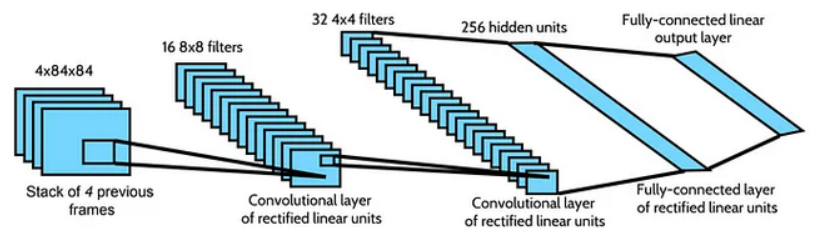
\includegraphics[width=0.75\linewidth]{image2.png}
    \caption{DQN CNN + Fully Connected General Architecture}
    \label{fig:enter-label}
\end{figure}

The architecture of this network consists of three convolutional layers followed by two fully connected layers.
This allows the agent to learn the policy directly from high-dimensional inputs and removes the need for manual feature extraction.

\subsubsection{DQN Architecture}

The DQN architecture follows the general framework of Q-learning, but the key distinction is that the Q-values are approximated using a neural network.

\vspace{-.5cm}\begin{figure}[H]
    \centering
    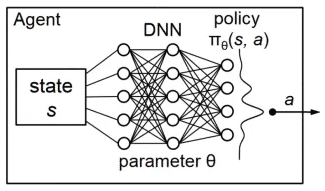
\includegraphics[width=0.4\linewidth]{dqnarch.png}
    \caption{DQN General Architecture}
    \label{fig:enter-label}
\end{figure}

The input to the network is a stack of 4 consecutive frames from an Atari game. The dimensions of each frame are 210×160. After they are preprocessed and stacked, the final dimensions are 4x84x84 when fed into the network. Four consecutive frames are used because a single frame cannot provide enough information about certain aspects of the environment that are necessary to make decisions, for example the velocity or acceleration of objects. These components need to be tracked across multiple frames, and thus, multiple frames need to be fed into the network.

The network contains two convolutional layers. These layers perform convolution operations to detect patterns in the pixel data. The first convolutional layer uses 16 8×8 filters, with a stride of 4, meaning the filters move 4 pixels at a time across the input. The second layer uses 32 4×4 filters and stride 2, so the filters move 2 pixels at a time. All of these layers use a ReLU activation function.

After the convolutional layers, the output is flattened into a 1D vector, which is passed to the fully connected layers. There are two of these fully connected layers, and they are used to process the learned features and produce Q-values for each action.
The first fully connected layer has 512 units, and the second has one unit for each possible action in the environment.
The output of the network is a vector of Q-values, where each element represents the total expected reward for taking each action in the given state.
The agent selects actions based on the Q-values, using an $\epsilon$-greedy policy, so the action with the highest Q-value is chosen. Sometimes random actions are chosen as well to encourage exploration during the general RL loop, as depicted in Figure \ref{fig:rlloop}.

\subsection{Experience Replay}
In normal Q-learning, the agent learns directly from sequential experiences, so the samples are highly correlated with each other.
This causes instability and makes training less efficient.
To counteract this, Experience Replay stores the agent’s experiences in a buffer, which is basically a memory of past experiences. Each experience is stored as a tuple, Experience=($s_{t},a_{t},r_{t},s_{t+1}$), where
$s_{t}$ is the state at time $t$, 
$a_{t}$ is the action taken at time $t$, 
$r_{t}$ is the reward received after taking action $a_{t}$, 
$s_{t+1}$ is the next state. During training, stochastic gradient descent is used and random mini-batches of experiences from the memory buffer are sampled.

The main benefit of the replay buffer is temporal correlations between experiences being broken. This is a result of random samples of experiences being used instead of just the most recent consecutive experiences. This results in the learning being more stable and generalizable because the network is trained on a bunch of past experiences that are not directly related to each other. As a result, the model will not try to exploit meaningless correlations in consecutive frames. Another benefit is improved data efficiency. Transitions in the replay buffer are reused multiple times each, as opposed to just once. Lastly, the chance of overfitting is reduced. There is enough variety in the sampled experiences that makes sure the model does not overfit to specific recent sequences of events like it would previously in normal Q-learning.

When using experience replay for learning, it must be done off-policy. This is required since the Q-network parameters in the current iteration are different than those in previous iterations which were used to generate a given sample, hence why an off-policy algorithm like Q-learning is used as the basis for DQN.

\begin{algorithm}
\caption{Deep Q-learning with Experience Replay\cite{dqn}}
\label{alg:DeepQlearningwithExperienceReplay}
\begin{algorithmic}[1]
    \State Initialize replay memory \( D \) to capacity \( N \)
    \State Initialize action-value function \( Q \) with random weights
    
    \For{episode \( = 1 \), \( M \)}
        \State Initialize sequence \( s_{1} = \{x_{1}\} \) and preprocessed sequenced \( \phi_{1} = \phi(s_{1}) \)
        \For{\( t = 1, T \)}
            \State With probability \( \epsilon \) select a random action \( a_{t} \)
            \State otherwise select \( a_{t} = \max_{a}Q*(\phi(s_{t}), a; \theta) \)
            \State Execute action at in emulator and observe reward \( r_{t} \) and image \( x_{t+1} \)
            \State Set \(s_{t+1} = s_{t}, a_{t}, x_{t+1} \) and preprocess \( \phi_{t+1} = \phi(s_{t+1}) \)
            \State Store transition (\( \phi_{t}, a_{t}, r_{t}, \phi_{t+1} \) ) in \( D \)
            \State Sample random minibatch of transitions (\( \phi_{j} , a_{j} , r_{j} , \phi_{j+1} \)) from \( D \)
            \State Set \( y_{j} = 
                \begin{cases} 
                  \text{\( r_{j} \)} & \text{for terminal \( \phi_{j+1} \)} \\
                  \text{\( r_{j} + \gamma \max_{a'}Q(\phi_{j+1},a';\theta)\)} & \text{for non-terminal \( \phi_{j+1} \)} \\
                \end{cases} \)
            \State Perform a gradient descent step on (\( y_{j} - Q(\phi_{j} , a_{j}; \theta))^{2} \) according to equation 12
        \EndFor
    \EndFor
\end{algorithmic}
\end{algorithm}

\subsection{Stabilizing Training with Separate Parameters}
Using fixed Q-Targets further helps to stabilize the learning process. The target for the Q-value update, $r_{t}+\gamma \max_{a'}Q'(s_{t+1},a';\theta^{-})$, is computed using a target network that is updated periodically rather than continuously. In this paper, the target network uses the weights from the previous iteration. A later paper extends this approach by allowing the target network to lag behind multiple iterations \cite{targetNetwork}. This periodic update prevents constantly changing Q-values and helps make learning more stable. In this paper, a single timestep is used, so the target at iteration $i$ would be calculated as:

\[y_{i} = \mathbb{E}_{s'\sim \mathcal{E}} [r + \gamma \max_{a'}Q(s', a'; \theta_{i-1})|s, a].\]

By keeping the target Q-values constant for a timestep, correlations between the Q-network and target-network are broken. This leads to better stability, as well as reducing oscillations and divergence during training.

\section{Paper Importance}
The introduction of Deep Q Networks through this paper was seen as a turning point in reinforcement learning research, and demonstrated that deep learning could be integrated with reinforcement learning to solve challenging problems. It led to the development of advanced algorithms such as DDPG (Deep Deterministic Policy Gradient) and SAC (Soft Actor-Critic). It also inspired further research into new directions in reinforcement learning, such as improving discrete methods, continuous control, and model-based reinforcement learning. 

\subsection{Results}
The paper showed that the same network architecture and hyperparameters could generalize across multiple games. This proved that the researchers' approach was not tailored to specific tasks, and opened the doors towards further innovations in this space. DQN achieved human-level performance or better in a variety of Atari games, including \textit{Pong}, \textit{Breakout}, and \textit{Enduro}. Each of these games have very different mechanics and goals. For instance, \textit{Pong} involves reflex-based paddle movement, \textit{Breakout} requires strategic brick-breaking, and \textit{Enduro} focuses on driving a car through a long-distance race environment. DQN was able to adapt to each of these different mechanics without needing to change its architecture or hyperparameters.

Additionally, when the predicted value function (Q curve) is plotted, it reflects the model's view of the environment. 

\begin{figure}[H]
    \centering
    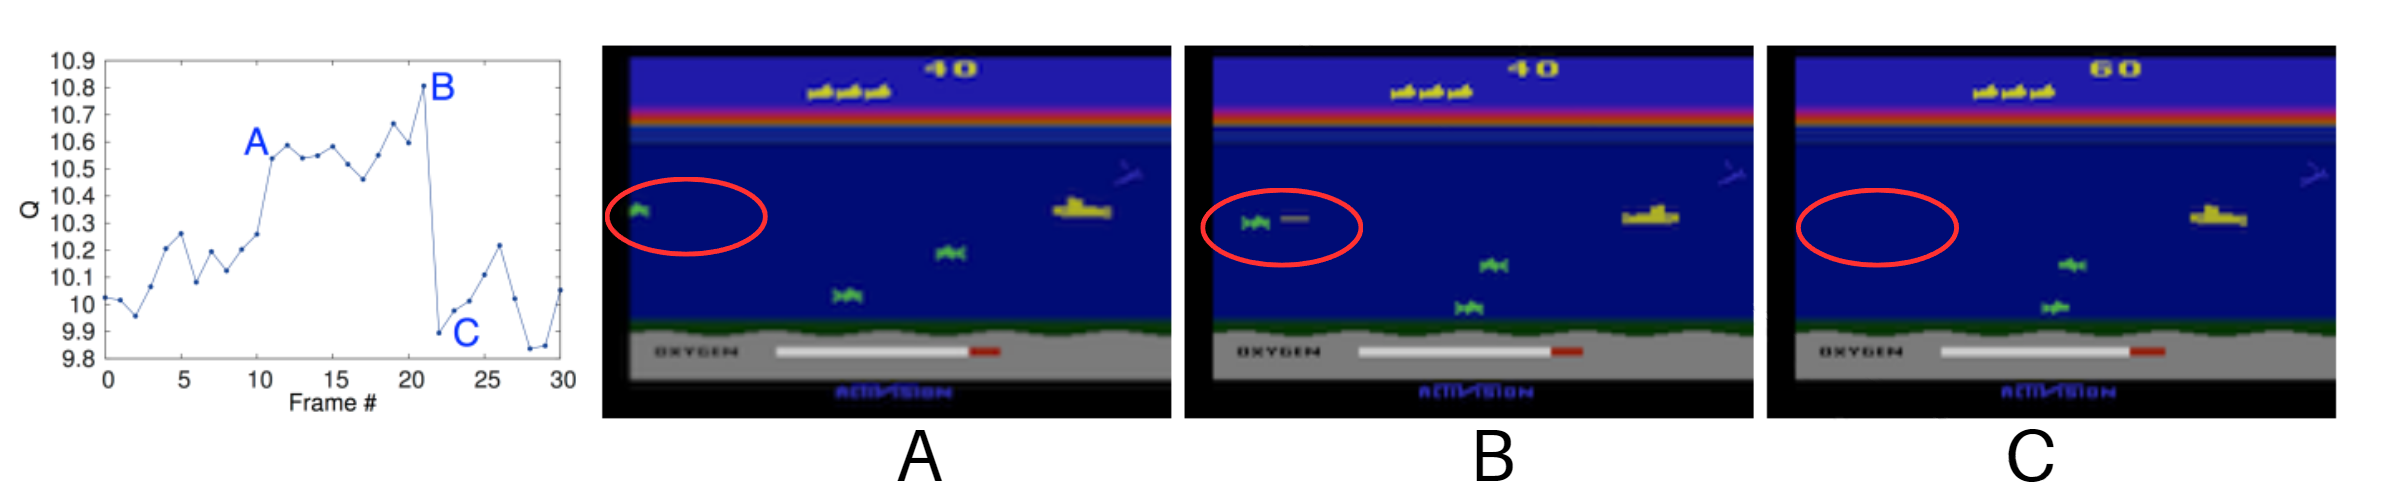
\includegraphics[width=0.75\linewidth]{qcurve.png}
    \caption{The leftmost plot shows the Q curve for a 30 second sequence for the game \textit{Seaquest}. The screens next to it correspond to the labeled frames, A, B, and C.}
    \label{fig:qcurve}
\end{figure}

\vspace{-0.5cm}As illustrated in Figure \ref{fig:qcurve} using the Atari game \textit{Seaquest}, the model's reward expectations fluctuate based on its interaction with the environment. When an enemy appears on the screen (Screen A), such as a fish, the model anticipates a high reward, which is reflected in a peak on the Q curve. Upon initiating an attack in response to the enemy (Screen B), the reward expectation increases slightly. Finally, once the enemy disappears (Screen C), signifying that the reward has been achieved, the reward expectation decreases. This sequence of events demonstrates how the model adapts and learns how to respond effectively to specific environmental cues. The model is able to do this because it learns to detect objects on its own through automated feature extraction. The researchers compared their results to results from other baseline methods, such as Sarsa, on features that were extracted manually, specific to the Atari task. Even though these features were specific to the task, these methods still had a lower performance than DQN, which extracted the features automatically.

DQN demonstrated the ability to extract features automatically on a large scale. The model’s raw input was frames of the Atari game screens, from which it automatically extracted the environment features. Through deep MLP architectures and their ability to perform automatic feature extraction, the agent can learn how to play games with complex state spaces efficiently while keeping the same architecture and learning process. 

\subsection{Limitations}
While this paper has vital concepts that are seen in reinforcement learning research today, it does not come without its limitations. The paper authors presented several limitations in their method that could be investigated in the future. 

DQN was designed only for discrete action spaces, a finite set of actions such as going up, down, left and right. It has difficulty with continuous actions, such as steering a vehicle. This is why DQN was tested with Atari games, as these games have a distinct set of input values that the Deep Q Network model can be used on. This limitation arises from the use of the Q-value function, which is computed for each discrete action. For continuous action spaces, there can be infinite action possibilities, and it becomes impossible to evaluate $Q(s,a)$ for every possible action.

This model can suffer from overestimation bias in its Q-function approximation. The update rule for Q-learning uses the maximum Q-value over all the possible actions that can happen at the next state, which has a tendency to overestimate the true value. This can be problematic in environments with stochastic transitions and rewards, such as game environments with random events, dealing with noise, or autonomous vehicles, where the state transitions and rewards are unpredictable. 

Training the model also requires millions of gameplay frames to converge to a suitable policy. The algorithm is computationally expensive and less suitable for environments where obtaining data is costly. For instance, real-world applications such as robotics or self-driving cars would need millions of pictures of the environment that the models are used in, which can be difficult and costly to obtain. 

DQN struggles with long-term planning. Its optimization strategy prioritizes immediate rewards, and can struggle when the best actions require long-term strategies, such as in tasks with delayed rewards. DQN relies on training the Q-network, which represents the Q-function. This requires it to learn a value function approximation, instead of just learning a policy. The reward function eventually converges to the same geometric sum after many steps, causing long term rewards to get lost in the process. This is evident in its less-than-human performance in games such as \textit{Q*bert}, \textit{Seaquest}, and \textit{Space Invaders}, whose winning strategy needs to be across longer time scales, as it takes a while to reach the first reward in these games. 

Finally, DQN is highly sensitive to hyperparameters, which include the learning rate, exploration rate, batch size, and the frequency of target network updates. Small changes in these parameters can lead to drastically difference learning outcomes, which can make DQN difficult to tune for new tasks or environments.  

\subsection{Relation to State of the Art Methods}
This paper led the groundwork for all modern reinforcement learning algorithms. Today's state of the art reinforcement learning methods build upon or address the limitations of DQN. Its contributions are fundamental concepts in these methods today. 

One of the prominent advancements from DQN is Soft Actor Critic (SAC) \cite{muzero}, a model-free reinforcement learning algorithm designed for continuous action spaces. Like DQN, model-free reinforcement learning algorithms take in raw inputs, not a model. SAC incorporates entropy regularization, which encourages exploration by adding a term that maximizes entropy alongside the reward signal. This helps SAC avoid premature convergence with suboptimal policies, improving its sample efficiency and exploration. SAC has superior performance in tasks with a high dimension of controls, directly addressing the continuous control limitation of DQN. 

Another important development is Twin-Delayed Deep Deterministic Policy Gradient (TD3) \cite{TD3}, which builds on Deep Deterministic Policy Gradient (DDPG) \cite{DDPG} by addressing overestimation bias. In DQN, overestimation occurs when the value of the next state-action pair is maximized in an unstable manner. TD3 mitigates this by using two Q-networks, and selecting the minimum Q-value from both of the Q-networks to avoid overestimation of the Q-value. Additionally, TD3 introduces delayed policy updates and target smoothing to improve stability during training. These modifications improve performance in complex environments with continuous action spaces, furthering the work done in DQN and overcoming its overestimation limitation. 

Trust-Region Policy Optimization (TRPO) \cite{TRPO} and Proximal Policy Optimization (PPO) \cite{PPO} are both designed to improve training instability, a major concern in DQN. TRPO was designed to prevent large policy updates that could destabilize training. It enforces a constraint on the step size of policy changes, using a trust region method. PPO, on the other hand, simplifies TRPO by using a clipped objective function that ensures that the policy does not deviate too drastically from the previous iteration. This stability makes PPO highly effective in both discrete and continuous control tasks, and it has been widely adopted in practice, especially in environments where stability and efficiency are necessary.

A more recent innovation, DreamerV3, \cite{dreamerv3} extends model-based reinforcement learning by combining pre-trained models of its environment with reinforcement learning. DreamerV3 learns a model of the environment that predicts future states and rewards, allowing the agent to plan actions more efficiently using its learned model rather than relying entirely on real-world interactions. This approach drastically reduces the amount of data needed to train the agent, making it more sample-efficient compared to DQN. It represents a significant step forward by blending model-based methods with the power of deep learning, addressing DQN’s computational inefficiency and making reinforcement learning more applicable to environments with high data costs.

Overall, the methods developed after DQN, such as SAC, TD3, TRPO, PPO, and DreamerV3, each build upon DQN’s foundational contributions but refine the process by handling the issues of sample inefficiency, overestimation bias, and continuous action spaces. These innovations extend the applicability of reinforcement learning, from video game environments to real-world tasks like robotic control, autonomous driving, and complex  decision-making, marking significant progress in the field.

\section{Conclusion}
This paper was fundamental to understanding the rise of deep reinforcement learning in artificial intelligence research history. It incorporated many components from our class, but it also allowed us to investigate new concepts such as how reinforcement learning actually works. Major areas to begin research in have already been investigated, as seen in several of the state of the art methods presented in the section above. The next step beyond this would be to tackle the long-term planning limitation, which is implicitly handled in DreamerV3, but is not quite entirely correct just yet. DQN was ultimately a groundbreaking step in the reinforcement learning field that opened the doors for new innovation. 

\subsection{Class Connection}
Through this paper, we learned a lot about reinforcement learning and how it can be connected with deep neural networks. In class, we investigated backpropagation and how it can be used to train a neural network, or in general any model with a layered architecture that can be represented as a computational graph. In this paper, we investigated the use of deep neural networks and backpropagation in reinforcement learning, as the DQN algorithm used deep neural networks for feature extraction, and backpropagation to update the Q-network. 

To understand this paper, we had to first tackle reinforcement learning, where we investigated the Bellman equations and their connection to DQN. Next, we had to understand Q-learning in order to understand the motivations behind DQN. Finally, we had to learn about the DQN architecture itself and how the choice to operate only as a function of the a state and produce a vector output of Q-value approximations allows it to fit into the Q-Learning algorithm, effectively replacing the Q-table. The process of learning the fundamental theory surrounding reinforcement learning overall required us to reform how we approach representation, evaluation, and optimization of problems, as well as make use of our understanding of basic probability theory.

\subsection{Paper Criticism}
While transformative in its research and findings, the authors overlooked some important components when writing this paper.

Further justification for certain design choices could have provided some much-needed insight into why things like experience replay and target networks were developed. These two components were key innovations presented in DQN, but the design choices behind them could have been addressed. For instance, they do not discuss why they chose the specific frequency of target network updates and the size of the replay buffer. The authors admit that DQN lacks any theoretical convergence guarantees, instead, they rely on their results to demonstrate that the model does converge. This reliance on empirical results, without a solid theoretical foundation, raises questions about the robustness of some of DQN's design choices. 

The authors also do not explicitly address the computational cost of DQN. It is implied when they mention that DQN was trained on 10 million frames, with a replay buffer of 1 million frames. This need for so much data is an implicit limitation that could have been addressed to contextualize the feasibility of DQN for researchers with limited computational resources to recreate their results. 

Finally, their experiments are only on Atari games and they only mention how DQN was designed for discrete control spaces. They do not address the performance in other domains, which leaves broader applications unclear, and provides another implicit limitation. 

These criticisms highlight areas where the paper could have provided more depth in explaining their contributions to the reinforcement learning field. While these criticisms do not diminish the importance of this paper in reinforcement learning research, addressing these concepts would have made the paper more comprehensive.  

\bibliographystyle{acm}
\bibliography{bibliography}
\end{document}